\documentclass{article}

% Language setting
% Replace `english' with e.g. `spanish' to change the document language
\usepackage[english]{babel}

% Set page size and margins
% Replace `letterpaper' with `a4paper' for UK/EU standard size
\usepackage[letterpaper,top=2cm,bottom=2cm,left=2cm,right=2cm,marginparwidth=1.75cm]{geometry}

% Useful packages
\usepackage{amsmath}
\usepackage{graphicx}
\usepackage[colorlinks=true, allcolors=blue]{hyperref}

\title{MATH285 Lab Report}
\author{Ren Jiashen , Zhou Zihan , Zheng Kaijun , Wu Dailin and Chen Jinyang}

\begin{document}

\begin{titlepage}
    \centering
    \vspace*{2cm}
    
    \Huge
    \textbf{ZJU-UIUC INSTITUTE}
    
    \vspace{0.5cm}
    \LARGE
    SP24 MATH285 Lab Report
    
    \vspace{1.5cm}
    
    \Large
    Group 15 Members:
    
    \vspace{0.5cm}
    \begin{minipage}{0.6\textwidth}
    \centering
    \begin{tabbing}
    Jiashen Ren \hspace{2cm} \= 322011 \\
    Zihan Zhou \> 322011 \\
    Jinyang Chen \> 322011 \\
    Kaijun Zheng \> 322011 \\
    Dailin Wu \> 322011 \\
    \end{tabbing}
    \end{minipage}

    \vspace{2cm}
    
    \Large
    \textbf{HONOR STATEMENT}
    
    \vspace{0.5cm}
    
    \normalsize
    We declare that this report is our own original work. For its preparation, we have not used any other resources than those cited as references. Every group member has a fair share in this work.
    
    \vspace{2cm}
    
    \begin{flushleft}
    \large
    Sign:
    
    \vspace{1.5cm}
    
    Date: 2024.5.25
    \end{flushleft}
    
\end{titlepage}

\maketitle

\begin{abstract}

This lab report aims to investigate the maximal solutions and their domains for two initial value problems (IVPs) using both numerical and analytical methods. The specific problems are as follows: 

\begin{equation*}
    \text{(IVP1)} \quad y' = y^2 - t^2, \quad y(0) = 1
\end{equation*}
\begin{equation*}
    \text{(IVP2)} \quad y' = y^3 - t^2y, \quad y(0) = 1
\end{equation*}

\end{abstract}

\section{Introduction}

This experiment focuses on solving two initial value problems (IVPs) using various numerical methods, including Euler, Improved Euler, and Runge-Kutta methods. We analyzed the performance of these methods by comparing their solutions for the given IVPs at different step sizes. Particular attention was paid to the behavior of the solutions near vertical asymptotes and accurately determining their positions at \( t = a_i, t = b_i, i = 1, 2 \).

Moreover, we explored alternative approaches to solving these problems. These included symmetry considerations, power series representations of the solutions, and simplifications of the differential equations through appropriate substitutions. The feasibility and accuracy of these alternative methods were also thoroughly examined. The results showed significant differences in the accuracy and efficiency of the various methods, with numerical methods proving to be highly reliable for complex initial value problems.

This report provides a detailed documentation of the computational processes and results obtained from each method. It also presents precise calculations for the vertical asymptotes of the solution graphs. These findings contribute to a better understanding and solution of similar differential equation initial value problems.


\section{Analysis Problem }

\subsection{Runge-Kutta method}

\subsubsection{Method}
Runge-Kutta methods are a class of iterative methods widely used for numerically solving ordinary differential equations (ODEs). Due to their high accuracy and applicability, especially the fourth-order Runge-Kutta method (RK4), they have been widely used in science and engineering. \\
Consider the initial value problem:
\[
y'(t) = f(t, y(t)), \quad y(t_0) = y_0
\]
The fourth-order Runge-Kutta method is used to compute the numerical solution from \( t_n \) to \( t_{n+1} = t_n + h \):

1. Compute the four slopes:
   \[
   k_1 = f(t_n, y_n)
   \]
   \[
   k_2 = f\left( t_n + \frac{h}{2}, y_n + \frac{h}{2} k_1 \right)
   \]
   \[
   k_3 = f\left( t_n + \frac{h}{2}, y_n + \frac{h}{2} k_2 \right)
   \]
   \[
   k_4 = f\left( t_n + h, y_n + h k_3 \right)
   \]

2. Update the value at the next time step:
   \[
   y_{n+1} = y_n + \frac{h}{6} (k_1 + 2k_2 + 2k_3 + k_4)
   \]
\subsubsection{Results Display}
1.For \[
y' = y^2 - t^2
\]

We detected a very large number at \( t = 1.0376 \), \( y = 6.800532522924118 \times 10^{18} \). 
\begin{figure}[h!]
    \centering
    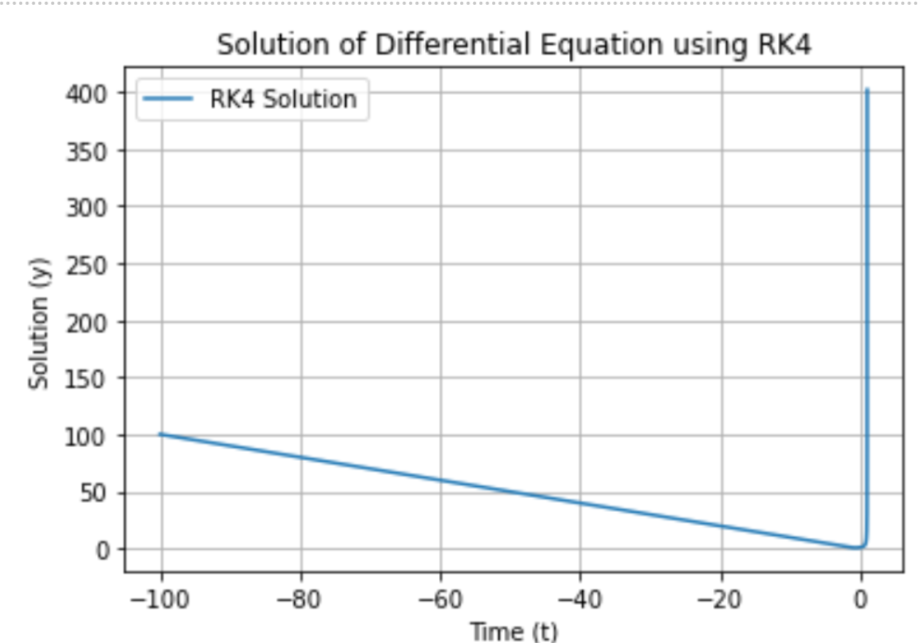
\includegraphics[width=0.5\linewidth]{pic学长/RK4_1.png}
    \caption{Result using RK4 method for the first function}
    \label{fig:example}
\end{figure}
We find that there is a breakpoint at the right end of the domain of definition with this function that should be very close to and slightly larger than \( t = 1.0376 \), while after simulation, there should be no restriction at the left end of the domain of definition and the function at the left end is very close to \( y = -x \).
2.For \[y' = y^3 - yt^2\]
\begin{figure}[h!]
    \centering
    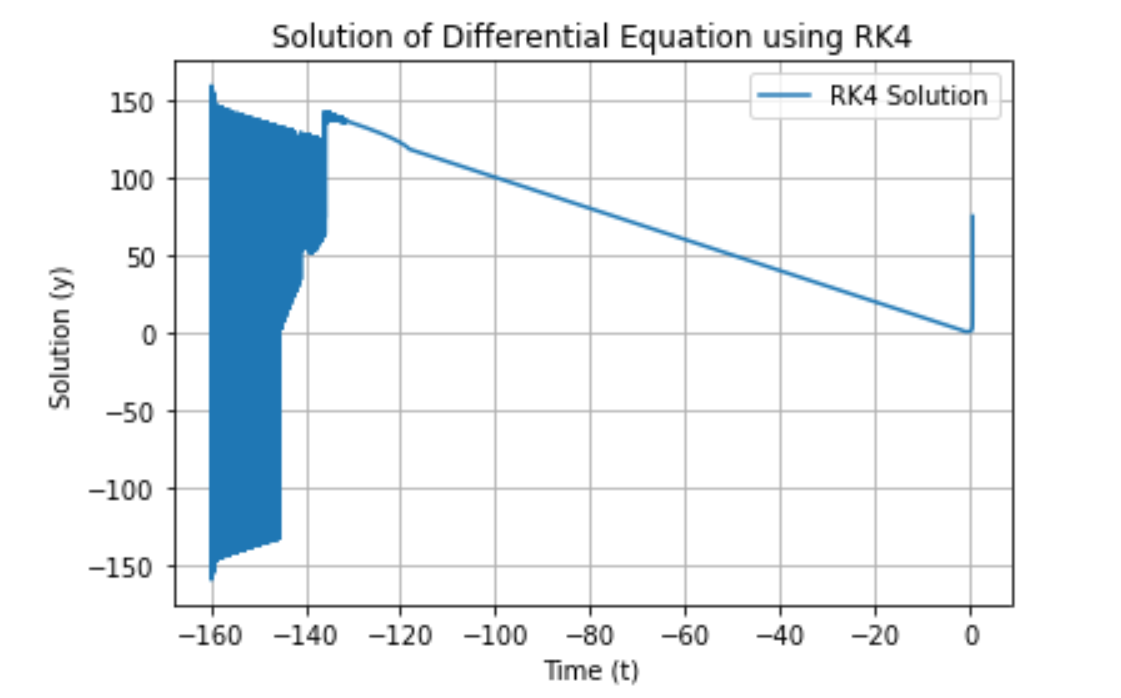
\includegraphics[width=0.5\linewidth]{pic学长/RK4_2.png}
    \caption{Result using RK4 method for the second function}
    \label{fig:example}
\end{figure}
We detected 2 very large numbers for this function, respectively  
at \( t=0.5112 \), \( y=3.797940674255831 \times 10^{41} \), and at \( t=-159.8557 \), \( y=1.250766724427035 \times 10^{24} \). 
So that there is a breakpoint at the right end of the domain of definition with this function that should be very close to and slightly larger than \( t = 0.5112 \). 
For the oscillations that appear on the left side, we speculate that they may be due to the effects of special functions such as the gamma function.
\subsubsection{Error Analysis}
The Taylor expansion of the exact solution at \( t_n \) is:
\[
y(t_{n+1}) = y(t_n + h) = y_n + hy'_n + \frac{h^2}{2!} y''_n + \frac{h^3}{3!} y'''_n + \frac{h^4}{4!} y''''_n + \mathcal{O}(h^5)
\]

Using \( y' = f(t, y) \), \( y'' = f_t + f_y y' \), etc., we can expand the derivatives as follows:

\[
y' = f(t, y)
\]
\[
y'' = \frac{\partial f}{\partial t} + \frac{\partial f}{\partial y} f
\]
\[
y''' = \frac{\partial^2 f}{\partial t^2} + 2 \frac{\partial^2 f}{\partial t \partial y} f + \frac{\partial^2 f}{\partial y^2} f^2 + \frac{\partial f}{\partial y} \left( \frac{\partial f}{\partial t} + \frac{\partial f}{\partial y} f \right)
\]
and so on.

We also expand the numerical solution:

\[
y_{n+1} = y_n + \frac{h}{6}(k_1 + 2k_2 + 2k_3 + k_4)
\]

where \( k_1 \), \( k_2 \), \( k_3 \), \( k_4 \) are:

\[
k_1 = f(t_n, y_n)
\]
\[
k_2 = f\left( t_n + \frac{h}{2}, y_n + \frac{h}{2} f(t_n, y_n) \right) \approx f(t_n, y_n) + \frac{h}{2} \left( \frac{\partial f}{\partial t} + \frac{\partial f}{\partial y} f \right)_{(t_n, y_n)} + \mathcal{O}(h^2)
\]
\[
k_3 = f\left( t_n + \frac{h}{2}, y_n + \frac{h}{2} k_2 \right) \approx f(t_n, y_n) + \frac{h}{2} \left( \frac{\partial f}{\partial t} + \frac{\partial f}{\partial y} k_2 \right)_{(t_n, y_n)} + \mathcal{O}(h^2)
\]
\[
k_4 = f(t_n + h, y_n + h k_3) \approx f(t_n, y_n) + h \left( \frac{\partial f}{\partial t} + \frac{\partial f}{\partial y} k_3 \right)_{(t_n, y_n)} + \mathcal{O}(h^2)
\]

Substitute these expansions into the numerical solution formula:

\begin{align*}
y_{n+1} &= y_n + \frac{h}{6} \bigg[ f(t_n, y_n) + 2\left( f(t_n, y_n) + \frac{h}{2} \left( \frac{\partial f}{\partial t} + \frac{\partial f}{\partial y} f \right) \right) \\
&\quad + 2\left( f(t_n, y_n) + \frac{h}{2} \left( \frac{\partial f}{\partial t} + \frac{\partial f}{\partial y} k_2 \right) \right) + f(t_n, y_n) + h \left( \frac{\partial f}{\partial t} + \frac{\partial f}{\partial y} k_3 \right) \bigg]
\end{align*}

Performing convergence analysis on the higher-order terms, we obtain:
\[
y_{n+1} - y(t_{n+1}) = \mathcal{O}(h^5)
\]

This shows that the local truncation error is \( \mathcal{O}(h^5) \).
\\
For Global Truncation Error,
While the local truncation error (LTE) at each step is \( \mathcal{O}(h^5) \), the global truncation error (GTE) considers the accumulation of these errors over many steps. 

For \( N = \frac{t_f - t_0}{h} \) steps, the global truncation error is given by summing up the local errors:

\[
\text{GTE} = \sum_{n=0}^{N-1} \mathcal{O}(h^5)
\]

Since there are \( N = \frac{t_f - t_0}{h} \) steps, the GTE can be approximated as:

\[
\text{GTE} = N \cdot \mathcal{O}(h^5) = \frac{t_f - t_0}{h} \cdot \mathcal{O}(h^5) = \mathcal{O}(h^4)
\]

Therefore, the global truncation error for the fourth-order Runge-Kutta method is \( \mathcal{O}(h^4) \).Therefore, the fourth-order Runge-Kutta method is highly accurate and very effective for numerically solving ordinary differential equations.


\subsection{Picard-Lindelof Iteration}

\subsubsection{Method}

The Picard method is an iterative approach for numerically solving initial value problems of ordinary differential equations. The core idea is to view the solution as a process of successive approximations, constructing a series of functions that converge to the true solution.

For the initial value problem:
\[
\frac{dy}{dt} = f(t, y), \quad y(t_0) = y_0
\]

The basic iterative formula of the Picard method is:
\[
y_{n+1}(t) = y_0 + \int_{t_0}^{t} f(\tau, y_n(\tau)) \, d\tau
\]

By repeatedly iterating this formula, we obtain a series of functions \( y_n(t) \) that progressively approximate the true solution.

\paragraph{Steps of the Picard Method}
\begin{enumerate}
    \item \textbf{Initial Condition:} Set \( y_0(t) = y_0 \) as the initial condition.
    \item \textbf{Iteration Process:}
    \[
    y_{n+1}(t) = y_0 + \int_{t_0}^{t} f(\tau, y_n(\tau)) \, d\tau
    \]
    By iterating this process multiple times, the sequence of functions \( \{y_n(t)\} \) converges to the true solution of the equation.
\end{enumerate}

\subsubsection{Results Display}

\paragraph{Solving Two Differential Equations with the Picard Method}

\subparagraph{Equation \( \frac{dy}{dt} = y^2 - t^2 \)}
For this equation, the Picard method's iterative formula is:
\[
y_{n+1}(t) = y_0 + \int_{t_0}^{t} (y_n(\tau))^2 - \tau^2 \, d\tau
\]

In each iteration, the integral of the previous iteration function \( y_n(t) \) is calculated. Due to the integral and squared term, this process may introduce significant errors, requiring multiple iterations to reduce the error.

\subparagraph{Equation \( \frac{dy}{dt} = y^3 - t^2 y \)}
For this equation, the Picard method's iterative formula is:
\[
y_{n+1}(t) = y_0 + \int_{t_0}^{t} (y_n(\tau))^3 - \tau^2 y_n(\tau) \, d\tau
\]

Due to the \( y^3 \) term, this problem can be more challenging, especially when \( y \) values are large, potentially causing steep slopes, increased computational instability, and error. In this case, the choice of iteration count and time step becomes crucial.

\clearpage

\begin{figure}[htbp]
    \centering
    \begin{minipage}[b]{0.45\textwidth}
        \centering
        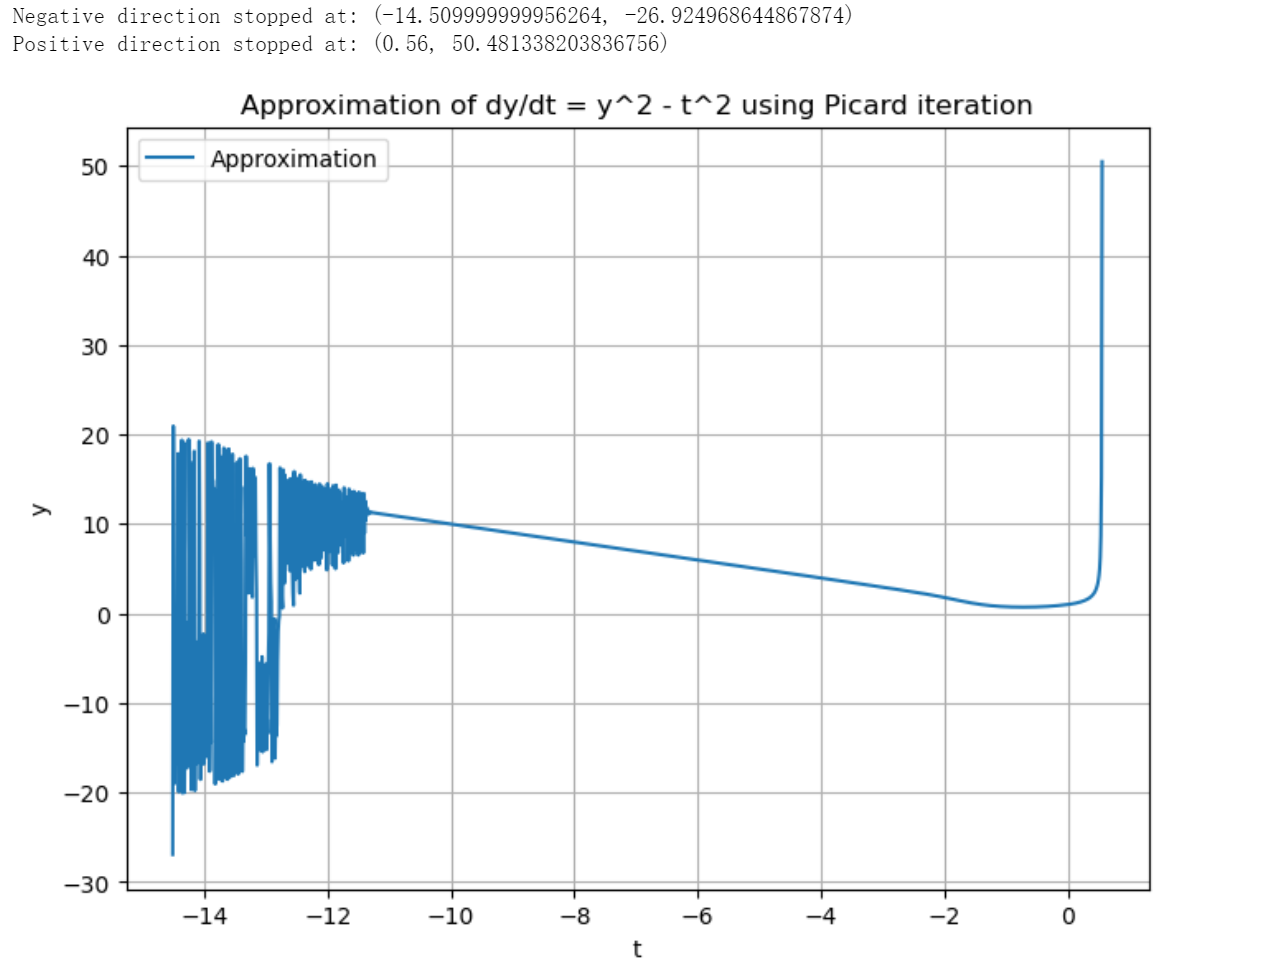
\includegraphics[width=\textwidth]{pic学长/2 (2).png }
        \caption{IVP 1}
        \label{fig:image1}
    \end{minipage}
    \hspace{0.05\textwidth}
    \begin{minipage}[b]{0.45\textwidth}
        \centering
        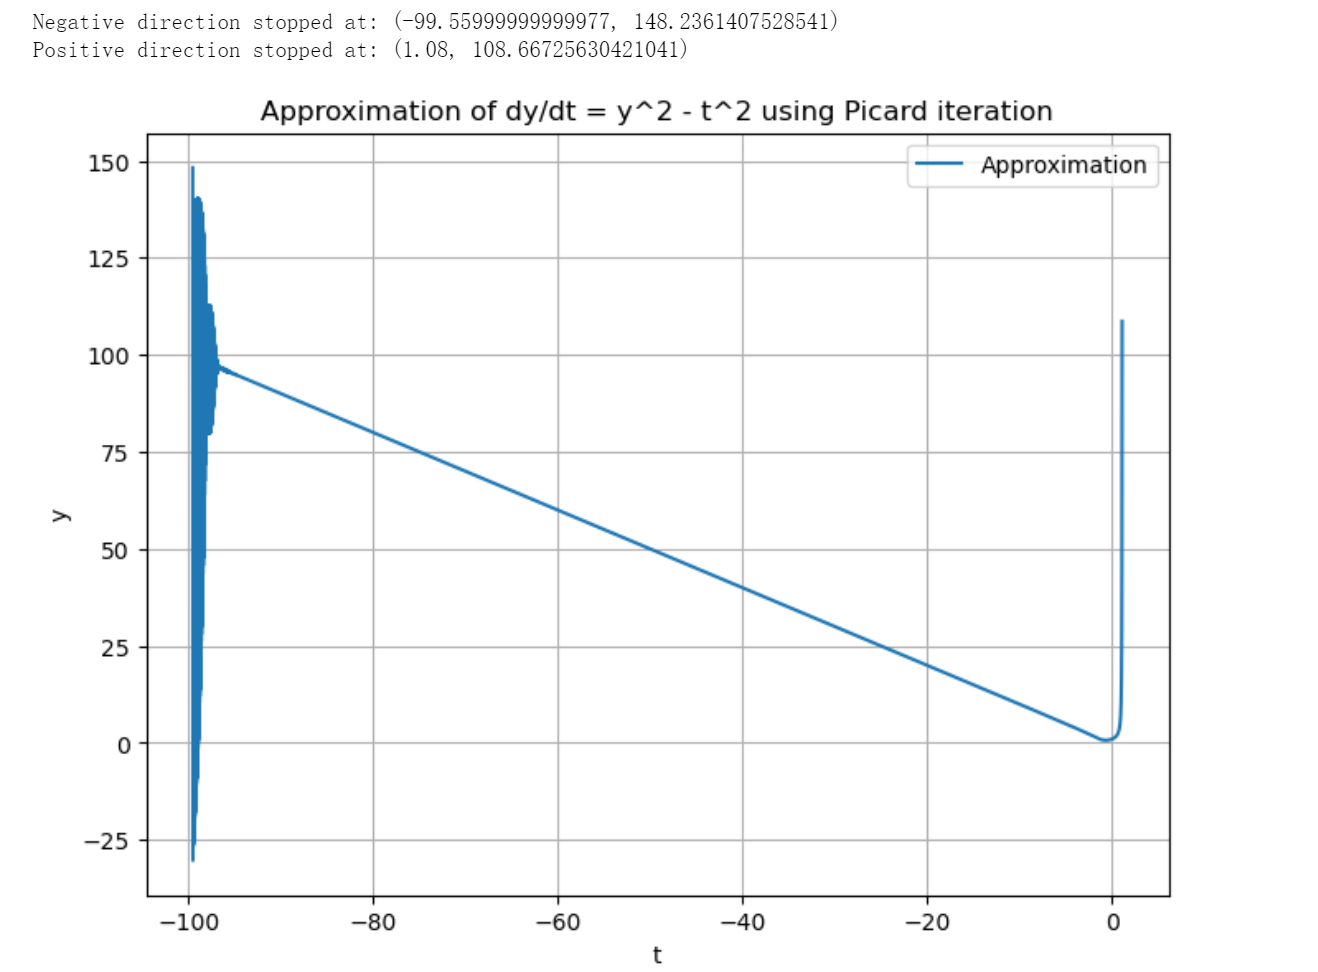
\includegraphics[width=\textwidth]{pic学长/3 (2).png}
        \caption{IVP 2}
        \label{fig:image2}
    \end{minipage}
\end{figure}


\subsubsection{Error Analysis}

The error analysis of the Picard method can be explained through the following points:

\paragraph{Initial Error}
Since the Picard method starts iterating from an initial approximation \( y_0 \), the choice of the initial approximation significantly affects the accuracy of the final solution.

\paragraph{Iteration Error}
Each iteration introduces an error, and these errors accumulate over the iterations, affecting the final solution's accuracy. The more iterations performed, the theoretically more accurate the solution becomes, but practical computation is limited by resources and rounding errors.

\paragraph{Convergence}
The convergence of the Picard method depends on the properties of the function \( f(t, y) \). For a Lipschitz continuous function \( f(t, y) \), the Picard method guarantees convergence. If \( f(t, y) \) does not satisfy the Lipschitz condition, the method may not converge or may converge very slowly.

\paragraph{Global Error}
The global error refers to the accumulated error from the initial condition \( y_0 \) to time \( t \). It is usually difficult to calculate precisely but can be reduced by decreasing the time step \( dt \) and increasing the number of iterations.

By understanding these principles and error control measures, the Picard method can be effectively used to solve different types of initial value problems for ordinary differential equations and control the associated errors.


\subsection{Series method}

\subsubsection{Method}
The series method is a powerful mathematical tool used to find analytic solutions to differential equations. This method assumes that the solution \( y(x) \) of the differential equation can be expressed in the form of a power series:
\[
y(x) = \sum_{n=0}^{\infty} a_n (x - x_0)^n
\]
where \( x_0 \) is the center of the power series expansion, and \( a_n \) are the coefficients to be determined.

To find the coefficients \( a_n \), the key steps of the series method include:

\begin{enumerate}
  \item \textbf{Computing Derivatives in Power Series Form}: \\
  Calculate the derivatives of \( y(x) \), such as \( y'(x) \) and \( y''(x) \), and express them in the power series form. For example, the first derivative of \( y(x) \) is given by:
  \[
  y'(x) = \sum_{n=1}^{\infty} n a_n (x - x_0)^{n-1}
  \]

  \item \textbf{Substituting into the Original Differential Equation}: \\
  Substitute the power series expressions of \( y(x) \) and its derivatives into the original differential equation. By aligning the powers on both sides of the equation, a recursive relation or direct formula for the coefficients \( a_n \) is obtained.

  \item \textbf{Using Initial or Boundary Conditions to Determine Coefficients}: \\
  Use the given initial or boundary conditions to determine the specific values of the coefficients \( a_n \), ensuring the uniqueness and correctness of the solution.
\end{enumerate}

Through this method, we can not only find the local solution of the differential equation near a specific point but also gain a deeper understanding of the nature and behavior of the solution. This is significant for both applied mathematics and theoretical research.


\subsubsection{Results Display}
\paragraph{Problem 1}
Following the above steps, we obtain the following recursive formula:
\[ \sum_{n=1}^{\infty} n a_n t^{n-1} = \sum_{n=0}^{\infty} \left( \sum_{k=0}^{n} a_k a_{n-k} \right) t^n - t^2 \] 

\begin{enumerate}
    \item For \( n=1 \)
       \[ a_1 = 1 \]
   Since \( y'(0) = a_1 \) and from the initial condition \( y'(0) = y(0)^2 - 0^2 = 1 \)
    \item For \( n \geq 2 \)
        \[ (n+1) a_{n+1} = \sum_{k=0}^{n} a_k a_{n-k} \] 
\end{enumerate}

\subparagraph{Conclusion}
The power series solution to the initial value problem is:
\[y(t) = 1 + t + t^2 + \frac{2t^3}{3} + \frac{5t^4}{6} + \frac{4t^5}{5} + \frac{23t^6}{30} + \frac{236t^7}{315} + \frac{201t^8}{280} + \frac{218t^9}{315} + \frac{2803t^{10}}{4200} + \ldots
\]

\paragraph{Problem 2}
The following recursive formula is obtained through the same algorithm:
\[
\sum_{n=0}^{\infty} (n+1) a_{n+1} t^n = \sum_{n=0}^{\infty} b_n t^n - \sum_{n=2}^{\infty} a_{n-2} t^n
\]
Matching the coefficients of the power series, we get the recurrence relation:
\[
(n+1) a_{n+1} = b_n - a_{n-2}
\]
where \( b_n \) is the coefficient of \( y^3(t) \).
The power series solution to the initial value problem is:
\[ y(t) = 1 + t + \frac{3}{2} t^2 + \frac{13}{6} t^3 + \cdots \]

\subsubsection{Error Analysis}

\begin{figure}[h]
    \centering
    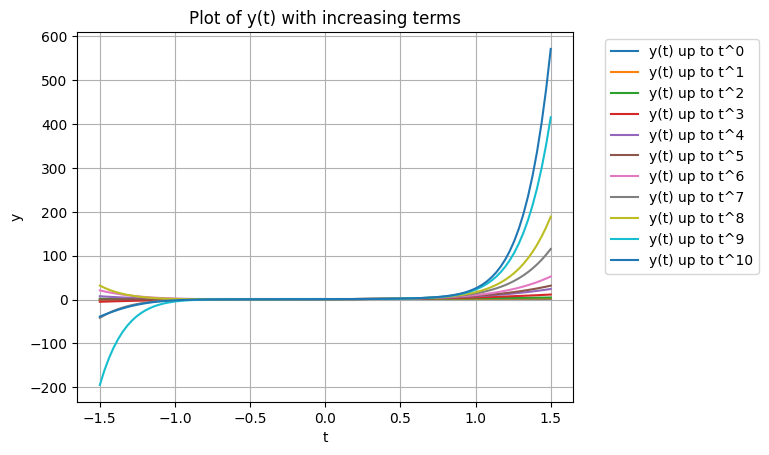
\includegraphics[width=0.6\linewidth]{pic学长/1.png}
    \caption{Series method for IVP 1}
    \label{fig:IVP 1}
\end{figure}

We found that as the number of terms in the expansion increases, the fitting accuracy of the function improves.However, for the second problem, since the number of expansion terms is relatively small, the solution only fits well near the initial value.



\subsection{Euler Method}

\subsubsection{Mathematical Analysis}

The Euler method is an explicit numerical integration method and a first-order method. Its basic idea is to use the slope at the current point to predict the value at the next point. For a given ordinary differential equation (ODE) \( y' = f(t, y) \) with initial condition \( y(t_0) = y_0 \), the Euler method's recurrence formula is:
\[
y_{n+1} = y_n + h f(t_n, y_n)
\]
where:
\begin{itemize}
    \item \( h \) is the step size;
    \item \( t_n = t_0 + nh \) is the current time step;
    \item \( y_n \) is the numerical solution at \( t_n \).
\end{itemize}

The mathematical foundation of the Euler method derives from the Taylor series expansion of \( y(t) \) at \( t_n \):
\[
y(t_{n+1}) = y(t_n) + h y'(t_n) + O(h^2)
\]
Neglecting the higher-order term \( O(h^2) \), the Euler method's approximation formula is obtained. The local truncation error is \( O(h^2) \), and the global truncation error is \( O(h) \).

The stability of the Euler method depends on the step size \( h \) and the properties of the differential equation. For stiff equations, the Euler method may require very small step sizes to remain stable, resulting in significantly increased computational cost.

\subsubsection{Result Presentation}

\begin{figure}[htbp]
    \centering
    \begin{minipage}[b]{0.45\textwidth}
        \centering
        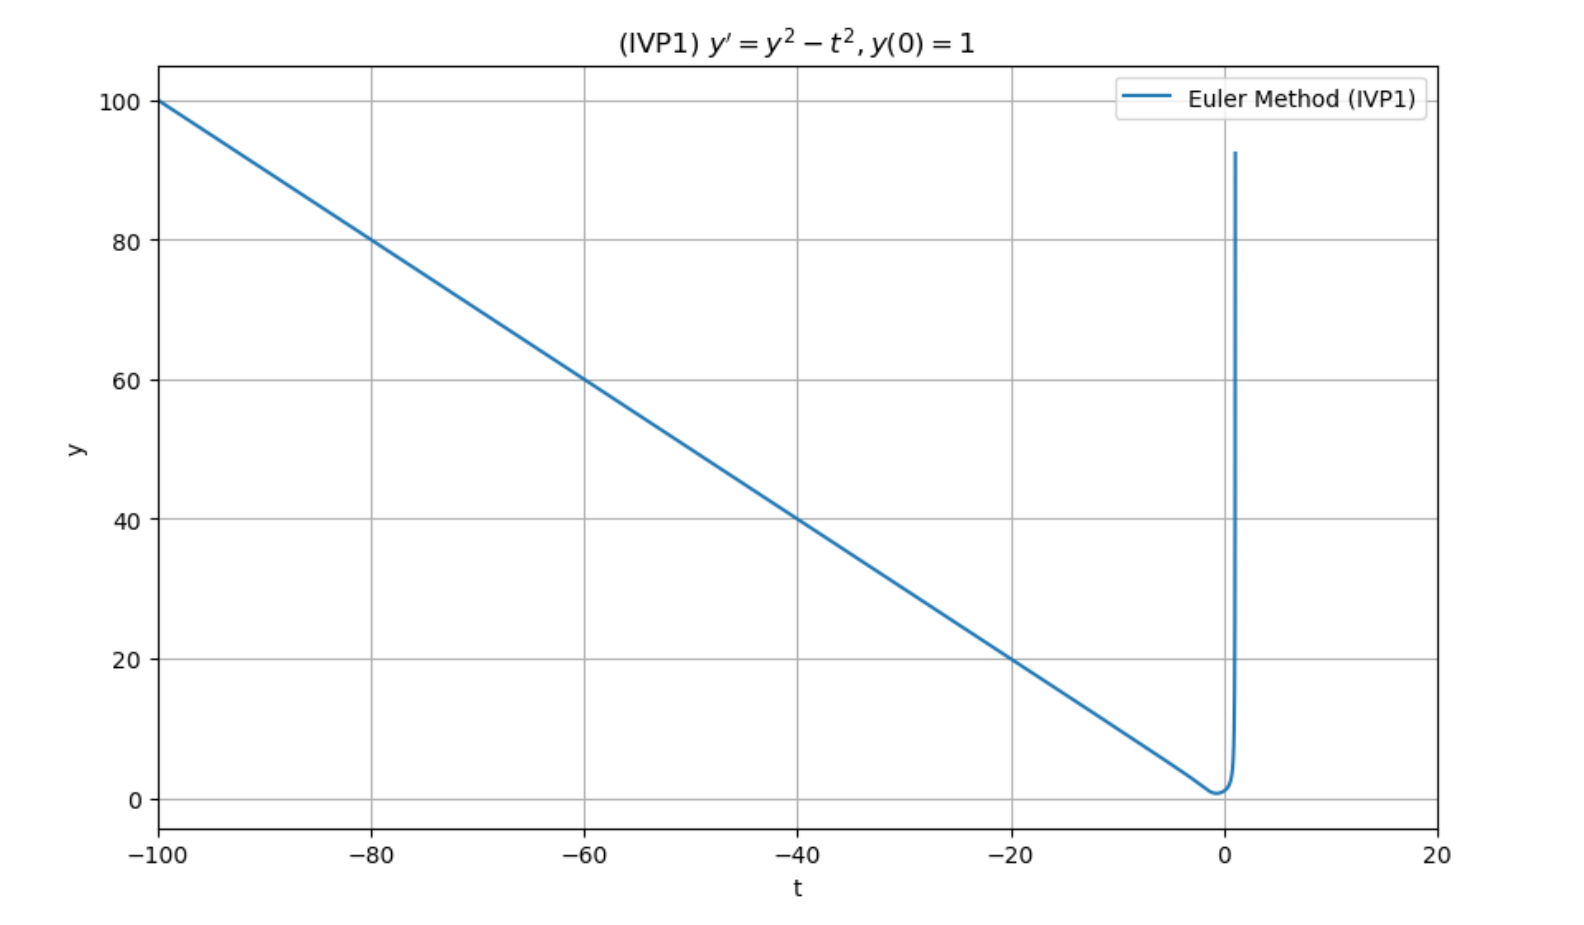
\includegraphics[width=\textwidth]{pic学长/欧拉方法-IVP1.png}
        \caption{Euler Method (IVP1)}
        \label{fig:image1}
    \end{minipage}
    \hspace{0.05\textwidth}
    \begin{minipage}[b]{0.45\textwidth}
        \centering
        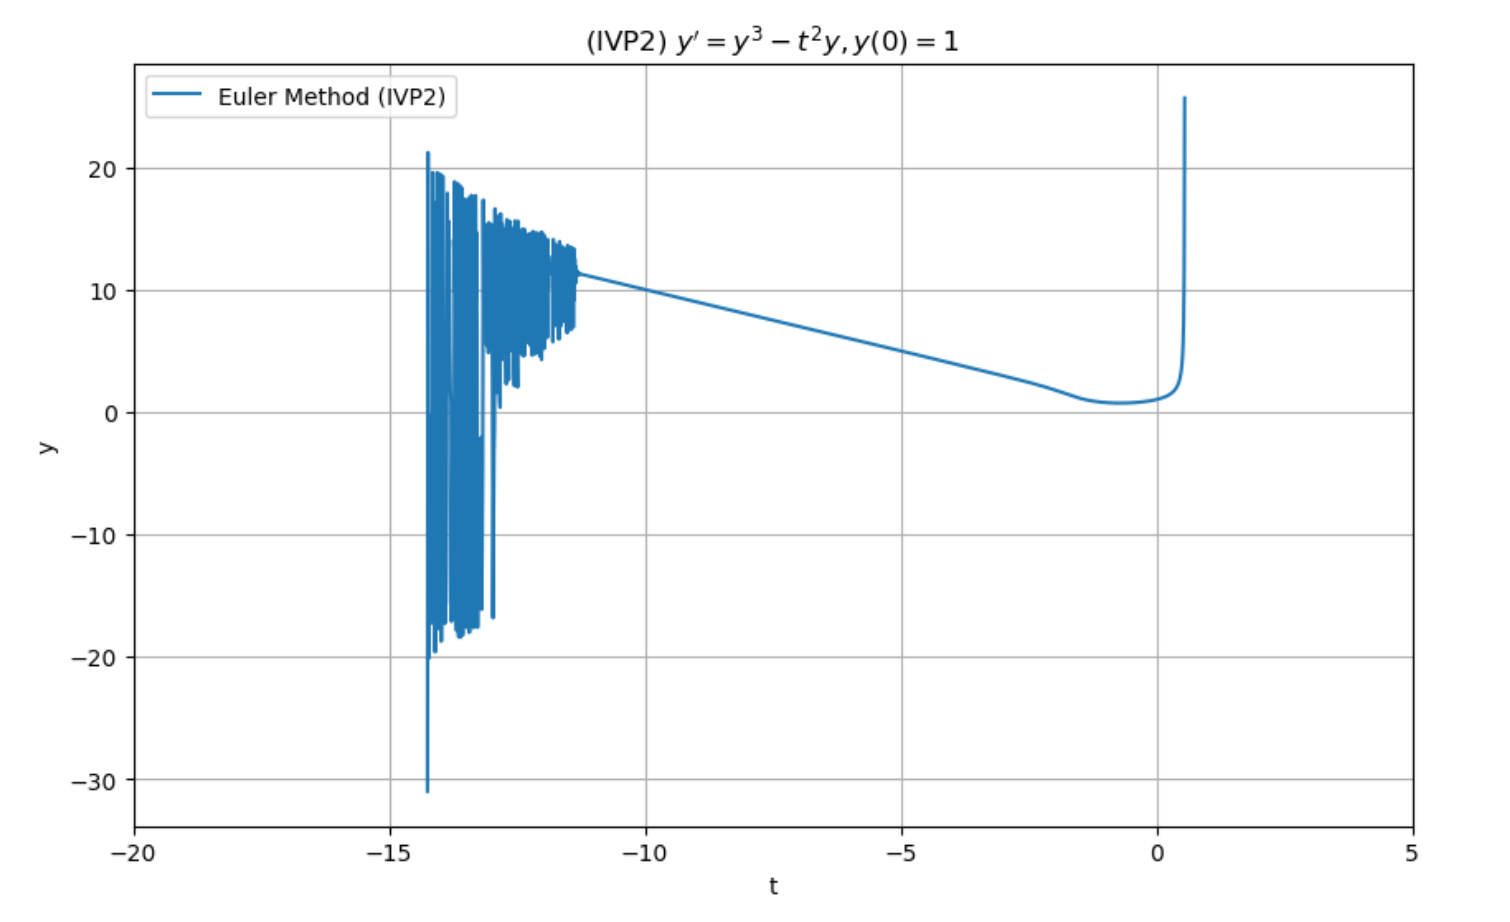
\includegraphics[width=\textwidth]{pic学长/欧拉方法-IVP2.png}
        \caption{Euler Method (IVP2)}
        \label{fig:image2}
    \end{minipage}
\end{figure}

\subsubsection{Error Analysis}
The error analysis of the Euler method focuses on its local and global truncation errors. The local truncation error is \( O(h^2) \), while the global truncation error is \( O(h) \). As a first-order method, the Euler method's error accumulates rapidly, especially when dealing with stiff problems, where the numerical solution may diverge quickly.

For (IVP1), the numerical solution shows a rapid increase as \( t \) approaches zero on the positive axis, indicating potential divergence. On the negative axis, the solution shows a linear downward trend with relatively minor errors.

For (IVP2), the solution exhibits significant oscillations on the negative axis, indicating instability in this region. This may be due to large numerical errors accumulating from a too-large step size.

\subsection{Improved Euler Method}

\subsubsection{Mathematical Analysis}
The improved Euler method (also known as the Heun method or trapezoidal method) enhances accuracy by incorporating the trapezoidal integration formula. The basic idea is to use the average slope between the current point and the predicted point to estimate the next point's value. For a given ODE \( y' = f(t, y) \) with initial condition \( y(t_0) = y_0 \), the improved Euler method's recurrence formula is:
\[
y_{n+1} = y_n + \frac{h}{2} \left[ f(t_n, y_n) + f(t_{n+1}, y_{n+1}^{\text{predict}}) \right]
\]
where:
\begin{itemize}
    \item \( y_{n+1}^{\text{predict}} = y_n + h f(t_n, y_n) \) is the Euler method prediction.
\end{itemize}

The improved Euler method can be viewed as applying the trapezoidal rule to the integration problem. By considering the average slope at two adjacent points, the local truncation error is \( O(h^3) \), and the global truncation error is \( O(h^2) \).

\subsubsection{Result Presentation}

\begin{figure}[htbp]
    \centering
    \begin{minipage}[b]{0.45\textwidth}
        \centering
        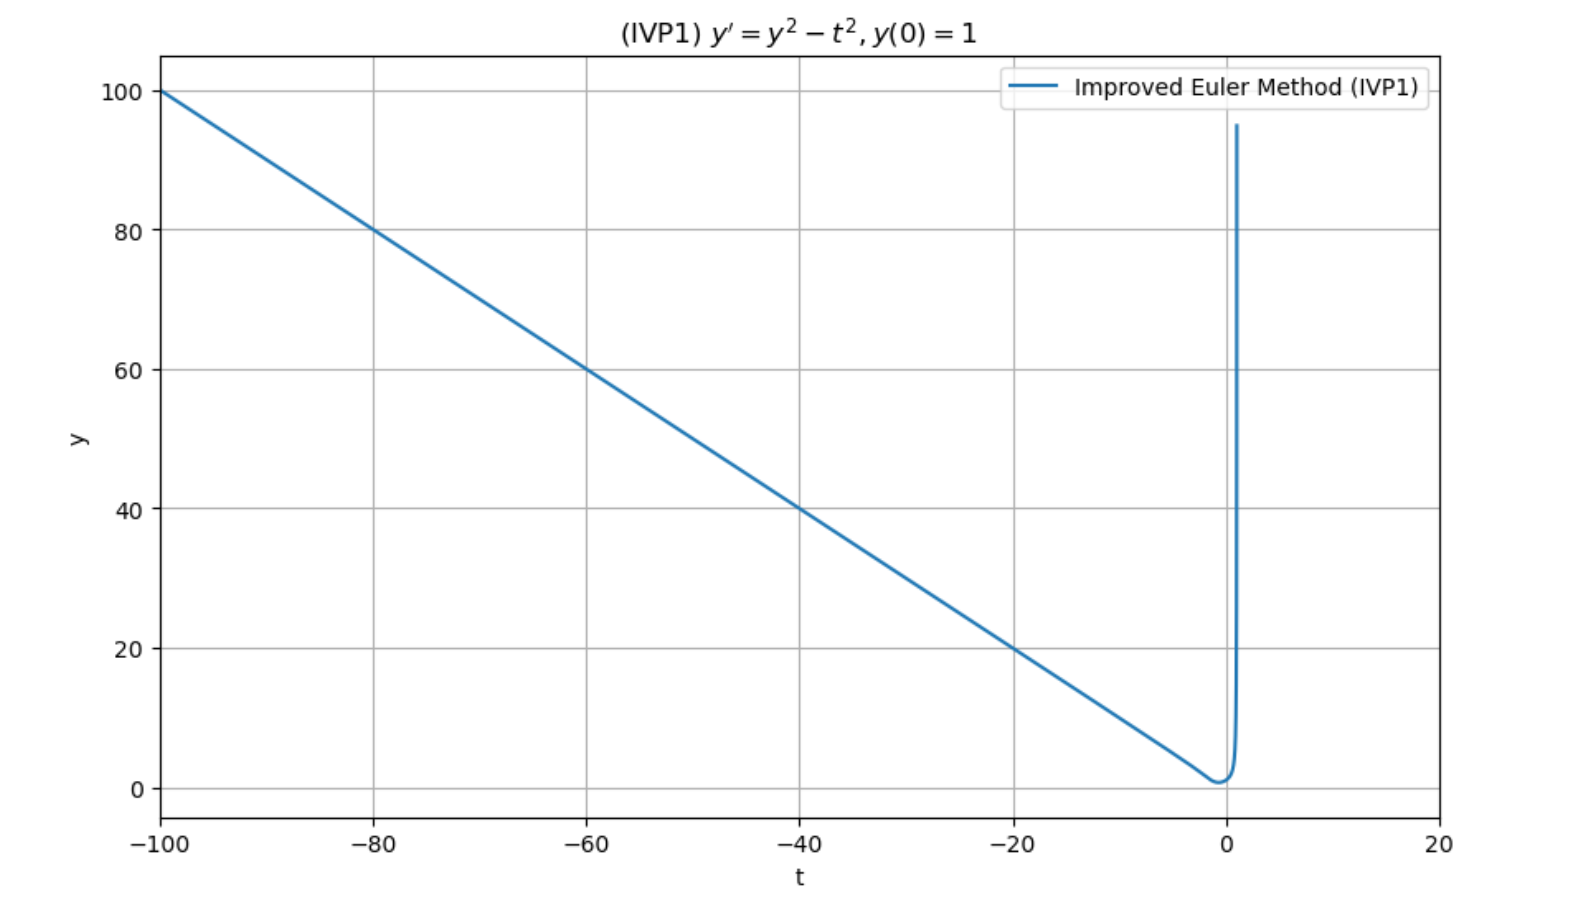
\includegraphics[width=\textwidth]{pic学长/改进欧拉方法-IVP1.png}
        \caption{Improved Euler Method (IVP1)}
        \label{fig:image1}
    \end{minipage}
    \hspace{0.05\textwidth}
    \begin{minipage}[b]{0.45\textwidth}
        \centering
        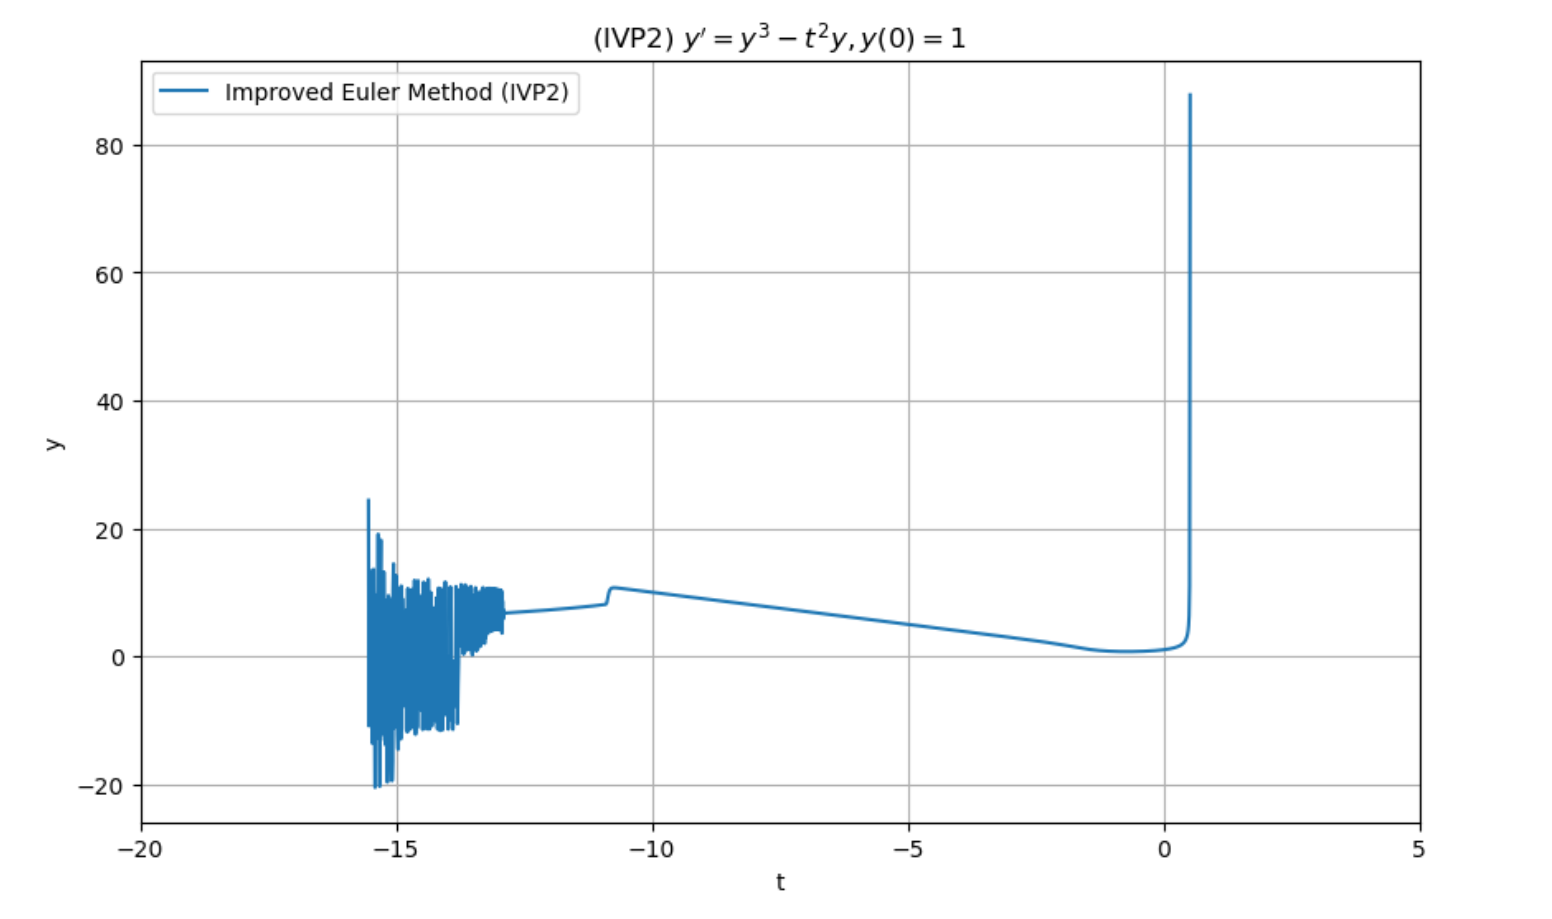
\includegraphics[width=\textwidth]{pic学长/改进欧拉方法-IVP2.png}
        \caption{Improved Euler Method (IVP2)}
        \label{fig:image2}
    \end{minipage}
\end{figure}

\subsubsection{Error Analysis}
The improved Euler method is a second-order method with a local truncation error of \( O(h^3) \) and a global truncation error of \( O(h^2) \). Compared to the Euler method, the improved Euler method is more stable when dealing with nonlinear and stiff problems. In this study, the improved Euler method shows higher accuracy and stability at the same step size, better capturing the solution's behavior.

For (IVP1), the improved Euler method produces a smoother solution near zero, and the linear downward trend on the negative axis is more pronounced, indicating reduced error.

For (IVP2), the improved Euler method still shows some oscillations on the negative axis, but the solution is more stable, and the error is reduced compared to the Euler method. This demonstrates the improved Euler method's advantage in handling complex nonlinear problems.

\subsubsection{Conclusion}
Compared with Euler Method, the numerical results indicate that the improved Euler method is superior in accuracy and stability, making it suitable for handling more complex differential equations. However, the choice of numerical method and step size should be based on the specific characteristics of the problem.

The comparative analysis shows that the improved Euler method can provide more stable and accurate solutions for problems with strong nonlinear terms. This further validates the importance and effectiveness of the improved Euler method in numerical computation.

In summary, although the improved Euler method requires slightly more computational effort than the Euler method, its higher accuracy and stability make it more advantageous in practical applications. Especially when dealing with complex and stiff problems, the improved Euler method significantly reduces numerical errors, providing more reliable solutions.
\subsection{Theoretical derivation}
\subsubsection{IVP 1}
We found that this equation is a special form of the Riccati Differential Equation. On page 87 of the book Elementary Differential Equations and Boundary Value Problems (4th ed., New York: Wiley, 1986) by W. E. Boyce and R. C. DiPrima, we found the relevant solution.
\[
y' = -t^2 + 0 \cdot y + 1 \cdot y^2
\]
Here \( P(t) = -t^2 \), \( Q(t) = 0 \), \( R(t) = 1 \).

Using the transformation \( y = -\frac{u'}{u} \), where \( R(t) = 1 \), we get:
\[
y = -\frac{u'}{u}
\]
Substituting this into the original equation, we get:
\[
\left( -\frac{u'}{u} \right)' = -t^2 + \left( -\frac{u'}{u} \right)^2
\]
Calculating the derivative, we get:
\[
\frac{u''u - (u')^2}{u^2} = -t^2 + \frac{(u')^2}{u^2}
\]
Simplifying this, we get:
\[
u'' + t^2 u = 0
\]

The generalized solution of this equation is:
\[
u(t) = c_1 D_{-\frac{1}{2}} \left( (1 + i)t \right) + c_2 D_{-\frac{1}{2}} \left( (-1 + i)t \right)
\]
We then used the computer to complete the subsequent calculations to get the results:

\begin{multline}
y(t) = \frac{\left( \frac{1}{2} + \frac{i}{2} \right)}{t \left[ \text{BesselJ}\left(\frac{1}{4}, \frac{it^2}{2}\right) \Gamma\left(\frac{1}{4}\right) - (1 + i)\sqrt{2} \text{BesselJ}\left(-\frac{1}{4}, \frac{it^2}{2}\right) \Gamma\left(\frac{3}{4}\right) \right]} \times \\
\left[ (-1 - i) t^2 \text{BesselJ}\left(-\frac{3}{4}, \frac{it^2}{2}\right) \Gamma\left(\frac{1}{4}\right) + i\sqrt{2} t^2 \text{BesselJ}\left(-\frac{5}{4}, \frac{it^2}{2}\right) \Gamma\left(\frac{3}{4}\right) \right. \\
\left. + \sqrt{2} \text{BesselJ}\left(-\frac{1}{4}, \frac{it^2}{2}\right) \Gamma\left(\frac{3}{4}\right) - i\sqrt{2} t^2 \text{BesselJ}\left(\frac{3}{4}, \frac{it^2}{2}\right) \Gamma\left(\frac{3}{4}\right) \right]
\end{multline}

\clearpage

\begin{figure}[htbp]
    \centering
    \begin{minipage}[b]{0.45\textwidth}
        \centering
        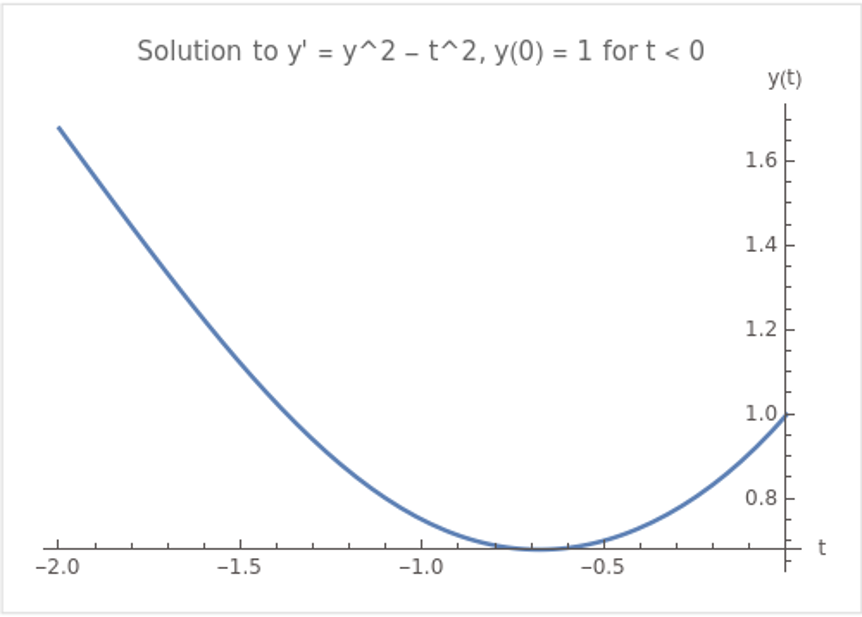
\includegraphics[width=\textwidth]{pic学长/图片1.png}
        \caption{IVP 1 when $t < 0$}
        \label{fig:image1}
    \end{minipage}
    \hspace{0.05\textwidth}
    \begin{minipage}[b]{0.45\textwidth}
        \centering
        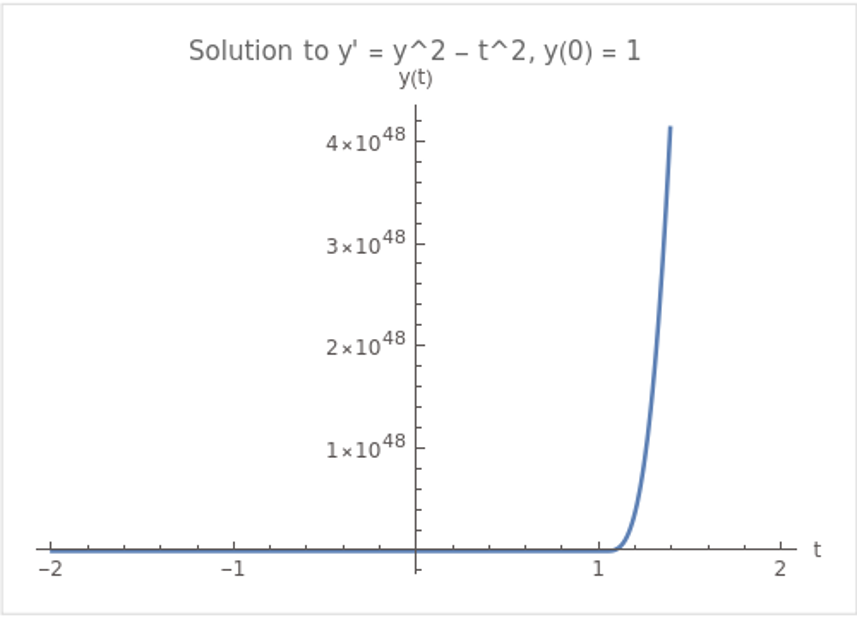
\includegraphics[width=\textwidth]{pic学长/图片2.png}
        \caption{IVP 1 when $t > 0$}
        \label{fig:image2}
    \end{minipage}
\end{figure}
\subsubsection{IVP 2}
Solve Bernoulli's equation \(\frac{dy(t)}{dt} = y(t)^3 - t^2 y(t)\), such that \(y(0) = 1\):

\[
\frac{dy(t)}{dt} + t^2 y(t) = y(t)^3
\]
Divide both sides by \(y(t)^3\):

\[
\frac{1}{y(t)^3} \frac{dy(t)}{dt} + \frac{t^2}{y(t)^2} = 1
\]

Let \(v(t) = \frac{1}{y(t)^2}\), which gives \(\frac{dv(t)}{dt} = -2 \frac{dy(t)}{dt} \frac{1}{y(t)^3}\):

\[
-2 \frac{dv(t)}{dt} t^2 v(t) = -2
\]

Let \(\mu(t) = e^{- \int -2 t^2 \, dt} = e^{- \frac{2}{3} t^3}\):

Multiply both sides by \(\mu(t)\):

\[
e^{-\frac{2}{3} t^3} \frac{d v(t)}{dt} - 2 t^2 e^{-\frac{2}{3} t^3} v(t) = -2 e^{-\frac{2}{3} t^3}
\]

Substitute \(-2 e^{-\frac{2}{3} t^3} t^2 = \frac{d}{dt}(e^{-\frac{2}{3} t^3})\):

\[
e^{-\frac{2}{3} t^3} \frac{d v(t)}{dt} + \frac{d}{dt} (e^{-\frac{2}{3} t^3}) v(t) = -2 e^{-\frac{2}{3} t^3}
\]

Apply the reverse product rule:

\[
\frac{d}{dt} (e^{-\frac{2}{3} t^3} v(t)) = -2 e^{-\frac{2}{3} t^3}
\]

Integrate both sides with respect to \(t\):

\[
\int \frac{d}{dt} (e^{-\frac{2}{3} t^3} v(t)) \, dt = \int -2 e^{-\frac{2}{3} t^3} \, dt
\]
Evaluate the integrals:

\[
e^{-(2t^3)/3} v(t) = \frac{\left(\frac{2}{3}\right)^{2/3} t \Gamma\left(\frac{1}{3}, \frac{2t^3}{3}\right)}{\sqrt[3]{t^3}} + c_1
\]

, where \( c_1 \) is an arbitrary constant.

\[
\text{Divide both sides by } \mu(t) = e^{-(2t^3)/3}:
\]

\[
v(t) = e^{(2t^3)/3} \left( \frac{\left(\frac{2}{3}\right)^{2/3} \sqrt[3]{3} t \Gamma\left(\frac{1}{3}, \frac{2t^3}{3}\right)}{\sqrt[3]{t^3}} + c_1 \right)
\]

Solve for \( y(t) \) in \( v(t) = \frac{1}{y(t)^2} \):

\[
y(t) = - \frac{\sqrt{3} \sqrt[6]{t^3}}{\sqrt{e^{(2t^3)/3} \left( \frac{\left(\frac{2}{3}\right)^{2/3} \sqrt[3]{3} t \Gamma\left(\frac{1}{3}, \frac{2t^3}{3}\right)}{\sqrt[3]{t^3}} + 3 c_1 \sqrt[3]{t^3} \right)}}
\]

or

\[
y(t) = \frac{\sqrt{3} \sqrt[6]{t^3}}{\sqrt{e^{(2t^3)/3} \left( \frac{\left(\frac{2}{3}\right)^{2/3} \sqrt[3]{3} t \Gamma\left(\frac{1}{3}, \frac{2t^3}{3}\right)}{\sqrt[3]{t^3}} + 3 c_1 \sqrt[3]{t^3} \right)}}
\]

By substituting the initial value \( y(0) = 1 \), we obtain the following results:

\begin{multline}
y(t) = \frac{\sqrt{3} \cdot t^{1/2}}{\sqrt{-\left( e^{\frac{2t^3}{3}} \left( -3t + 2^{2/3} \cdot 3^{1/3} \cdot \Gamma \left( \frac{1}{3} \right) - 2^{2/3} \cdot 3^{1/3} \cdot t \cdot \Gamma \left( \frac{1}{3}, \frac{2t^3}{3} \right) \right) \right)}}
\end{multline}

\paragraph{Asymptotes and analysis of stability}
We found that there was a surge in the function at \( t \approx 0.5112 \), and we guessed that there might be a non-primitive function in the solution.Since the gamma function appears as a singularity on the negative semiaxis, in essence the second function on the negative semiaxis is not well-defined.

\begin{figure}[htbp]
    \centering
    \begin{minipage}[b]{0.45\textwidth}
        \centering
        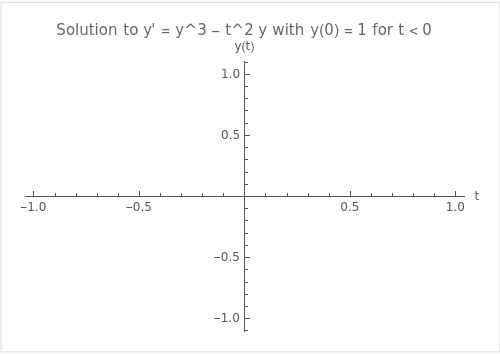
\includegraphics[width=\textwidth]{pic学长/图片3.png}
        \caption{IVP 2 when $t < 0$}
        \label{fig:image1}
    \end{minipage}
    \hspace{0.05\textwidth}
    \begin{minipage}[b]{0.45\textwidth}
        \centering
        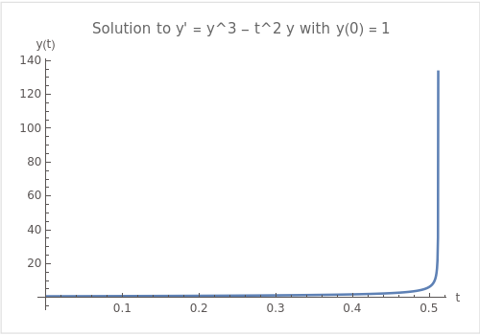
\includegraphics[width=\textwidth]{pic学长/图片4.png}
        \caption{IVP 2 when $t > 0$}
        \label{fig:image2}
    \end{minipage}
\end{figure}


\section{Conclusion}

In this lab report, we thoroughly explored the solutions to two initial value problems (IVPs) using both numerical and analytical methods. Specifically, we applied Euler, Improved Euler, Runge-Kutta, Picard-Lindelof iteration, and the Series method to solve the IVPs:

\begin{equation*}
    \text{(IVP1)} \quad y' = y^2 - t^2, \quad y(0) = 1
\end{equation*}
\begin{equation*}
    \text{(IVP2)} \quad y' = y^3 - t^2y, \quad y(0) = 1
\end{equation*}

We applied several numerical methods, including Euler, Improved Euler, Picard-Lindelof Iteration, and Runge-Kutta (RK4), to approximate the solutions. Our analysis focused on the behavior of solutions near the vertical asymptotes.For (IVP1), the RK4 method provided accurate solutions up to t=1.0376, indicating a vertical asymptote. For (IVP2), the RK4 method identified significant points at t=0.5112, suggesting vertical asymptotes. The sharp oscillations in the left part also reflect the fact that the solution of the function is a non-simple function and there may be problems with the domain of definition.

Theoretical analysis was a key part of our investigation.
We first tried the Series method and got crude results.Then, for (IVP1), we identified the equation as a special form of the Riccati Differential Equation. By using the transformation and solving the resulting second-order differential equation, we derived the exact solution with the help of computer.
For (IVP2), we transformed the equation into a Bernoulli's equation and used the method of integrating factors to find the exact solution.

In conclusion, this study emphasizes the significance of combining numerical methods with rigorous theoretical analysis to solve IVPs effectively. The insights gained from both approaches enhance our understanding and provide robust tools for tackling similar problems in future research.
\end{document}